\documentclass[tikz,border=8pt]{standalone}
\usepackage[T1]{fontenc}
\usepackage{amsmath,amssymb}
\usepackage{xcolor}
\usepackage{tikz}
% Shared TikZ style for the DEV architecture diagrams.
% Requires only TikZ and standard TikZ libraries.
\usetikzlibrary{arrows.meta,backgrounds,calc,fit,positioning}

\definecolor{DevInk}{HTML}{172033}
\definecolor{DevMuted}{HTML}{526078}
\definecolor{DevLine}{HTML}{475569}
\definecolor{DevPanel}{HTML}{F8FAFC}
\definecolor{DevPanelBorder}{HTML}{CBD5E1}
\definecolor{DevContent}{HTML}{DBEAFE}
\definecolor{DevContentBorder}{HTML}{2563EB}
\definecolor{DevStyle}{HTML}{F3E8FF}
\definecolor{DevStyleBorder}{HTML}{9333EA}
\definecolor{DevStable}{HTML}{DCFCE7}
\definecolor{DevStableBorder}{HTML}{16A34A}
\definecolor{DevAllograph}{HTML}{FFEDD5}
\definecolor{DevAllographBorder}{HTML}{EA580C}
\definecolor{DevCritic}{HTML}{FEE2E2}
\definecolor{DevCriticBorder}{HTML}{DC2626}
\definecolor{DevLoss}{HTML}{FEF3C7}
\definecolor{DevLossBorder}{HTML}{D97706}

\tikzset{
  devtext/.style={font=\sffamily\small, text=DevInk, align=center},
  devbox/.style={
    devtext,
    draw=DevPanelBorder,
    fill=white,
    rounded corners=2.2mm,
    line width=0.75pt,
    inner xsep=3.2mm,
    inner ysep=2.4mm,
    minimum height=9mm
  },
  devinput/.style={devbox, draw=DevContentBorder, fill=DevContent},
  devcontent/.style={devbox, draw=DevContentBorder, fill=DevContent},
  devstyle/.style={devbox, draw=DevStyleBorder, fill=DevStyle},
  devstable/.style={devbox, draw=DevStableBorder, fill=DevStable},
  devallograph/.style={devbox, draw=DevAllographBorder, fill=DevAllograph},
  devcritic/.style={devbox, draw=DevCriticBorder, fill=DevCritic},
  devloss/.style={devbox, draw=DevLossBorder, fill=DevLoss},
  devgroup/.style={
    draw=DevPanelBorder,
    fill=DevPanel,
    rounded corners=3mm,
    line width=0.75pt,
    inner sep=4mm
  },
  devflow/.style={
    -{Latex[length=2.8mm,width=1.9mm]},
    draw=DevLine,
    line width=0.85pt,
    rounded corners=1.4mm
  },
  devaux/.style={
    devflow,
    draw=DevStableBorder,
    densely dashed
  },
  devlossflow/.style={
    devflow,
    draw=DevLossBorder,
    densely dashed
  },
  devlabel/.style={
    font=\sffamily\scriptsize,
    text=DevMuted,
    fill=white,
    inner sep=1.2pt
  },
  devgrouptitle/.style={
    font=\sffamily\bfseries\small,
    text=DevInk,
    fill=DevPanel,
    inner xsep=2mm,
    inner ysep=0.6mm
  },
  devnote/.style={
    font=\sffamily\scriptsize,
    text=DevMuted,
    align=left
  }
}



\begin{document}
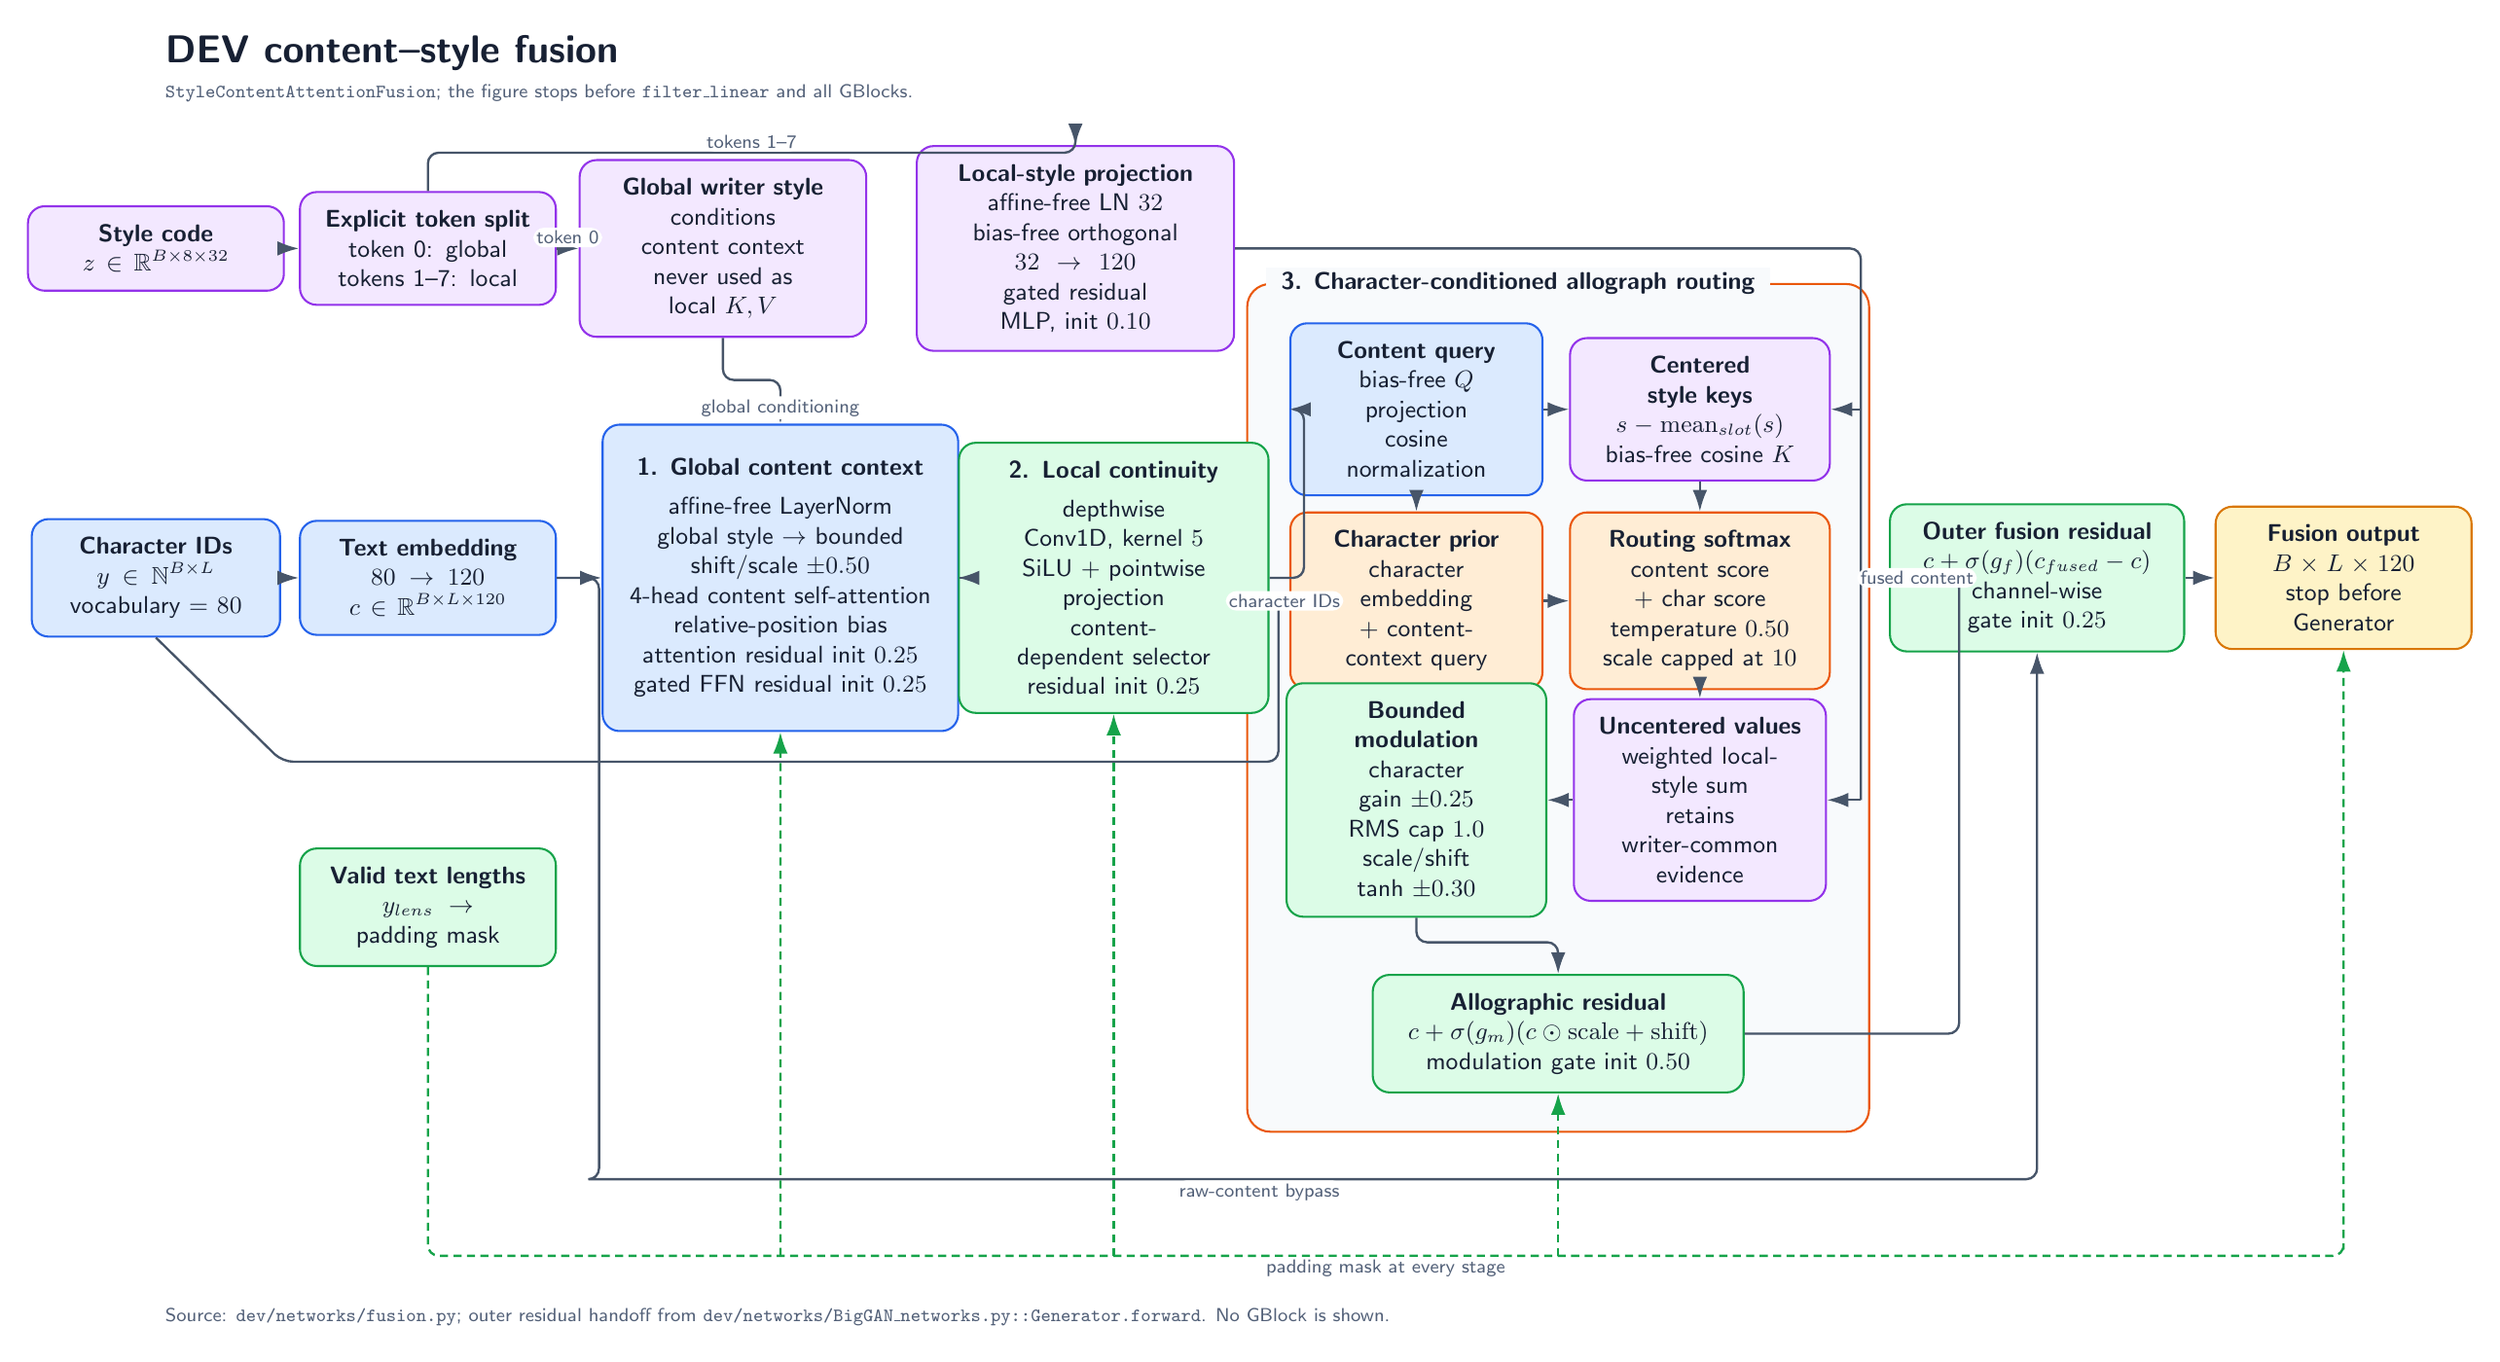
\begin{tikzpicture}[x=1cm,y=1cm]
  \node[font=\sffamily\bfseries\Large, text=DevInk, anchor=west]
    at (0,13.3) {DEV content--style fusion};
  \node[devnote, anchor=west]
    at (0,12.78) {\texttt{StyleContentAttentionFusion}; the figure stops before \texttt{filter\_linear} and all GBlocks.};

  % Style lane. Global and local tokens have separate contracts from the split.
  \node[devstyle, text width=2.7cm] (stylecode) at (0,10.75)
    {\textbf{Style code}\\$z\in\mathbb{R}^{B\times8\times32}$};
  \node[devstyle, text width=2.7cm] (split) at (3.55,10.75)
    {\textbf{Explicit token split}\\token 0: global\\tokens 1--7: local};
  \node[devstyle, text width=3.1cm] (globalstyle) at (7.4,10.75)
    {\textbf{Global writer style}\\conditions \mbox{content context}\\never used as local $K,V$};
  \node[devstyle, text width=3.5cm] (localproj) at (12.0,10.75)
    {\textbf{Local-style projection}\\affine-free LN $32$\\bias-free \mbox{orthogonal} $32\rightarrow120$\\gated residual MLP, init $0.10$};

  \draw[devflow] (stylecode) -- (split);
  \draw[devflow] (split) -- node[devlabel,above] {token 0} (globalstyle);
  \coordinate (splitLocalLane) at (3.55,12.00);
  \coordinate (localProjLane) at (12.00,12.00);
  \draw[devflow] (split.north) -- (splitLocalLane) -- node[devlabel,above] {tokens 1--7} (localProjLane) -- (localproj.north);

  % Content input lane.
  \node[devinput, text width=2.6cm] (charids) at (0,6.45)
    {\textbf{Character IDs}\\$y\in\mathbb{N}^{B\times L}$\\vocabulary $=80$};
  \node[devcontent, text width=2.7cm] (embedding) at (3.55,6.45)
    {\textbf{Text embedding}\\$80\rightarrow120$\\$c\in\mathbb{R}^{B\times L\times120}$};
  \node[devstable, text width=2.7cm] (lengths) at (3.55,2.15)
    {\textbf{Valid text lengths}\\$y_{lens}\rightarrow$ padding mask};

  \draw[devflow] (charids) -- (embedding);

  % Stage 1 and Stage 2 use compact boxes so the main content path is a single,
  % uninterrupted horizontal lane.
  \node[devcontent, text width=4.0cm, minimum height=4.0cm] (stageone) at (8.15,6.45)
    {\textbf{1. Global content context}\\[1.2mm]
     affine-free LayerNorm\\
     global style $\rightarrow$ bounded shift/scale $\pm0.50$\\
     4-head content self-attention\\
     relative-position bias\\
     attention residual init $0.25$\\
     gated FFN residual init $0.25$};
  \node[devstable, text width=3.4cm, minimum height=3.25cm] (stagetwo) at (12.50,6.45)
    {\textbf{2. Local continuity}\\[1.2mm]
     depthwise Conv1D, kernel $5$\\
     SiLU + \mbox{pointwise} projection\\
     content-dependent selector\\
     residual init $0.25$};

  \draw[devflow] (embedding) -- (stageone);
  \draw[devflow] (stageone) -- (stagetwo);
  \draw[devflow] (globalstyle.south) -- ++(0,-0.55) -| node[devlabel,pos=0.82] {global conditioning} (stageone.north);

  % Stage 3: all paths have dedicated columns. The local-style bus runs around
  % the right edge of the stage, never through a node.
  \node[devcontent, text width=2.65cm] (query) at (16.45,8.65)
    {\textbf{Content query}\\bias-free $Q$ projection\\cosine \mbox{normalization}};
  \node[devstyle, text width=2.75cm] (keys) at (20.15,8.65)
    {\textbf{Centered style keys}\\$s-\mathrm{mean}_{slot}(s)$\\bias-free cosine $K$};
  \node[devallograph, text width=2.65cm] (charprior) at (16.45,6.15)
    {\textbf{Character prior}\\character embedding\\+ content-context query};
  \node[devallograph, text width=2.75cm] (routing) at (20.15,6.15)
    {\textbf{Routing softmax}\\content score + char score\\temperature $0.50$\\scale capped at $10$};
  \node[devstyle, text width=2.65cm] (values) at (20.15,3.55)
    {\textbf{Uncentered values}\\weighted local-style sum\\retains \mbox{writer-common} evidence};
  \node[devstable, text width=2.75cm] (bounded) at (16.45,3.55)
    {\textbf{Bounded modulation}\\character gain $\pm0.25$\\RMS cap $1.0$\\scale/shift tanh $\pm0.30$};
  \node[devstable, text width=4.2cm] (modres) at (18.30,0.50)
    {\textbf{Allographic residual}\\$c+\sigma(g_m)(c\odot\mathrm{scale}+\mathrm{shift})$\\modulation gate init $0.50$};

  \draw[devflow] (stagetwo.east) -- ++(0.45,0) |- (query.west);
  \draw[devflow] (query) -- (keys);
  \draw[devflow] (query.south) -- (charprior.north);
  \draw[devflow] (charprior) -- (routing);
  \draw[devflow] (keys.south) -- (routing.north);
  \draw[devflow] (routing.south) -- (values.north);
  \draw[devflow] (values) -- (bounded);
  \draw[devflow] (bounded.south) -- ++(0,-0.32) -| (modres.north);

  % Local-style bus: top horizontal lane and right vertical lane.
  \coordinate (localbusTop) at (22.25,10.75);
  \coordinate (localbusKey) at (22.25,8.65);
  \coordinate (localbusValue) at (22.25,3.55);
  \draw[draw=DevLine,line width=0.85pt,rounded corners=1.4mm]
    (localproj.east) -- (localbusTop) -- (localbusValue);
  \draw[devflow] (localbusKey) -- (keys.east);
  \draw[devflow] (localbusValue) -- (values.east);

  % Character-ID lane travels below Stage 1/2 and enters only the character prior.
  \coordinate (charlaneA) at (1.65,4.05);
  \coordinate (charlaneB) at (14.65,4.05);
  \draw[devflow] (charids.south) -- (charlaneA) -- (charlaneB) |- node[devlabel,pos=0.78] {character IDs} (charprior.west);

  % Final fusion handoff. Raw content uses a dedicated lower bypass lane.
  \node[devstable, text width=3.2cm] (outergate) at (24.55,6.45)
    {\textbf{Outer fusion residual}\\$c+\sigma(g_f)(c_{fused}-c)$\\channel-wise gate init $0.25$};
  \node[devloss, text width=2.7cm] (fusionout) at (28.55,6.45)
    {\textbf{Fusion output}\\$B\times L\times120$\\stop before Generator};

  \draw[devflow] (modres.east) -- ++(2.80,0) |- node[devlabel,pos=0.80] {fused content} (outergate.west);
  \draw[devflow] (outergate) -- (fusionout);

  \coordinate (rawA) at (5.70,-1.40);
  \coordinate (rawB) at (23.1,-1.40);
  \draw[devflow] (embedding.east) -- ++(0.55,0) |- (rawA) -- node[devlabel,below] {raw-content bypass} (rawB) -| (outergate.south);

  % Padding mask occupies its own lowest lane, separated from the raw-content bypass.
  \coordinate (maskA) at (3.55,-2.40);
  \coordinate (maskB) at (28.55,-2.40);
  \draw[devaux] (lengths.south) -- (maskA) -- node[devlabel,below] {padding mask at every stage} (maskB) -| (fusionout.south);
  \draw[devaux] ($(maskA)+(4.60,0)$) -- (stageone.south);
  \draw[devaux] ($(maskA)+(8.95,0)$) -- (stagetwo.south);
  \draw[devaux] ($(maskA)+(14.75,0)$) -- (modres.south);

  \begin{scope}[on background layer]
    \node[devgroup, draw=DevAllographBorder,
      fit=(query)(keys)(charprior)(routing)(values)(bounded)(modres), inner sep=5mm] (stage3group) {};
  \end{scope}
  \node[devgrouptitle, anchor=west] at ($(stage3group.north west)+(0.25,0)$)
    {3. Character-conditioned allograph routing};

  \node[devnote, anchor=west] at (0,-3.20)
    {Source: \texttt{dev/networks/fusion.py}; outer residual handoff from \texttt{dev/networks/BigGAN\_networks.py::Generator.forward}. No GBlock is shown.};
\end{tikzpicture}
\end{document}

